\paragraph*{Learned cross-resource allocation under mixed disturbances.}
The supplementary attention analysis makes the interaction patterns behind the heterogeneous representation visible (Figures~\ref{fig:attn-change} and \ref{fig:attn-types}). It uses the \texttt{dense\_i1\_mix\_start5\_min8\_cause4\_opt\_main\_seed42} checkpoint, with 96 test samples per condition selected deterministically with episode stratification. Normal samples have neither a current nor a future bottleneck; upcoming samples have no current bottleneck but at least one future bottleneck; ongoing samples have at least one current bottleneck. Resource weights are averaged over samples, history steps, heads and encoder layers, with dropout inactive. For readability, all resource-level heatmaps display the 20 machine, gantry, human and AGV nodes and omit the 18 buffer rows and columns without renormalizing the retained values. The corresponding absolute matrices are retained in Appendix~\ref{app:absolute-attention}.

Subtracting the normal-condition average in Figure~\ref{fig:attn-change} removes the persistent attention backbone and exposes the localized redistribution associated with upcoming and ongoing bottlenecks. The type-level summary in Figure~\ref{fig:attn-types} makes interactions among machines, gantries, humans and AGVs easier to inspect. Each cell is a mean over a query-type/attended-type block, not the total attention mass assigned to that type; group sizes differ. These views describe how heterogeneous information is used in the supplementary checkpoints. The configuration comparisons above, rather than attention magnitude, quantify predictive benefit.
\zhpara{图~\ref{fig:attn-change}与图~\ref{fig:attn-types}补充展示混合扰动模型如何利用异构资源信息；对应的绝对注意力矩阵移至附录~\ref{app:absolute-attention}。分析使用 \texttt{dense\_i1\_mix} 的五分钟 checkpoint，每种状态依据 episode 分层确定性选取九十六个测试样本。正常状态指当前和未来均无瓶颈；即将发生指当前无瓶颈而未来至少出现一个；进行中指当前至少存在一个瓶颈。资源注意力对样本、历史时间、头和编码层取均值，推理时关闭 dropout。为提高可读性，资源级热力图仅显示二十个机器、龙门、人员和 AGV 节点，省略十八个缓冲区的行列，保留数值不重新归一化。图~\ref{fig:attn-change}减去正常状态均值，从稳定的注意力骨架中分离出与瓶颈状态相关的局部重新分配；类型图汇总四类被显示资源之间的关系。类型单元格是资源块的均值，而非分配到该类型的总权重，各类资源数量也不相同。注意力用于描述信息分配，预测收益仍由前述配置对照支持，不能由注意力大小推断因果贡献。}
\begin{figure*}[p]
\centering
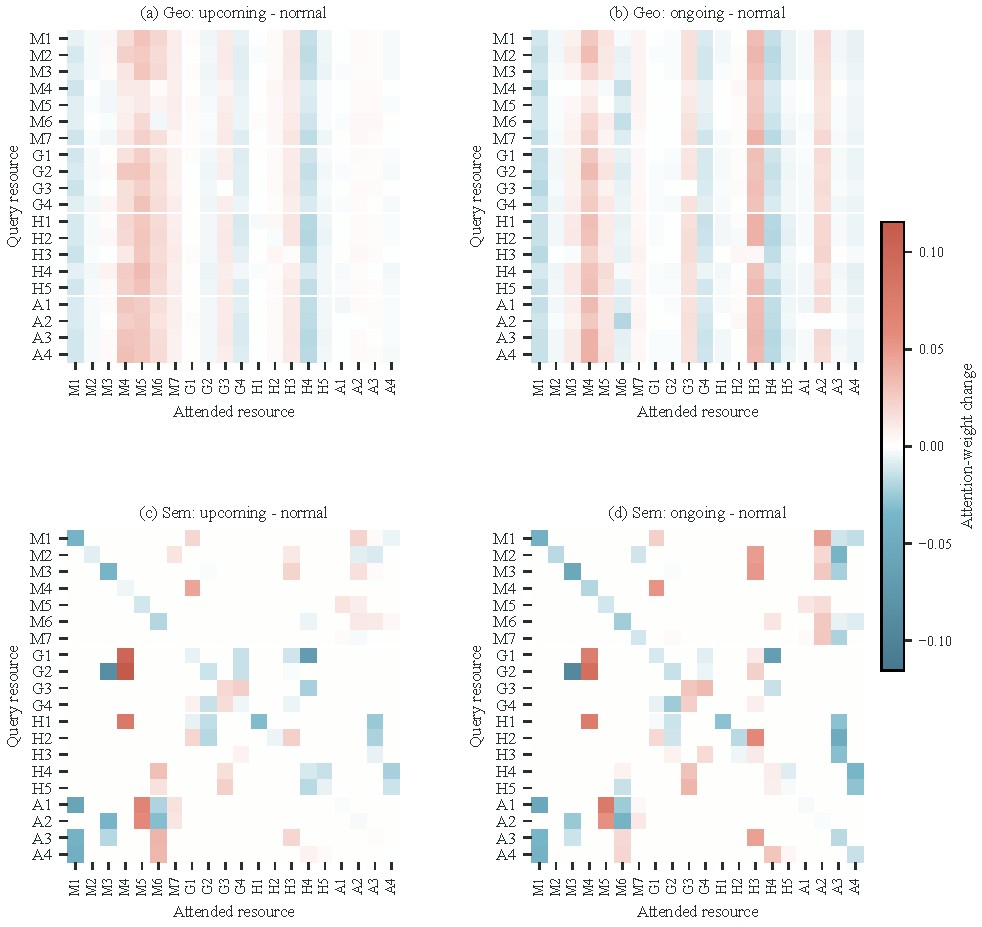
\includegraphics[width=0.98\textwidth,height=0.78\textheight,keepaspectratio]{figures/attention_heatmaps/fig03_resource_attention_change.pdf}
\caption{Resource-attention redistribution relative to normal operation for upcoming and ongoing samples. The displayed matrices retain 20 machine, gantry, human and AGV nodes; 18 buffer nodes are omitted without renormalization. Coral denotes increased weight and blue decreased weight on the shared signed scale; near-yellow cells are approximately unchanged. These are changes in associative weights, not intervention effects. Start cap 5 min; 96 selected samples per condition; averages cover history steps, heads and layers. Mixed-disturbance supplementary analysis (\texttt{dense\_i1\_mix}, seed 42); not the retained \texttt{dense\_i1} evaluation.}
\label{fig:attn-change}
\end{figure*}
\begin{figure*}[p]
\centering
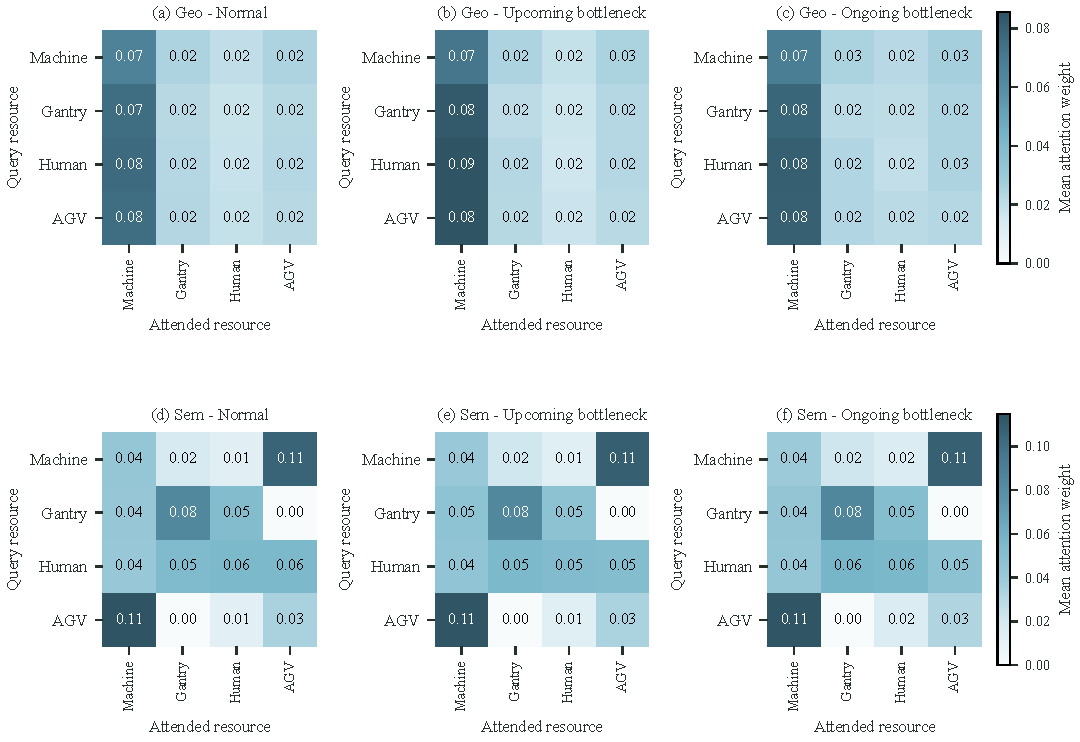
\includegraphics[width=0.98\textwidth,height=0.78\textheight,keepaspectratio]{figures/attention_heatmaps/fig06_entity_type_attention.pdf}
\caption{Attention summarized over the four displayed resource types under the three conditions; buffer nodes are omitted. Each value is the mean of a query-type/attended-type block; unequal type sizes prevent interpreting it as total type importance. Geographic and semantic rows have separate scales. Mixed-disturbance supplementary analysis (\texttt{dense\_i1\_mix}, seed 42); not the retained \texttt{dense\_i1} evaluation.}
\label{fig:attn-types}
\end{figure*}
